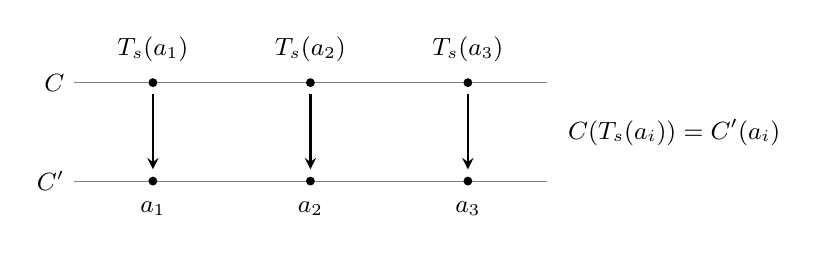
\begin{tikzpicture}[x=1cm,y=1cm,>=stealth, every node/.style={font=\small}]
 \draw[gray] (0,1.25) -- (6,1.25);
 \draw[gray] (0,0) -- (6,0);
 \node[anchor=east] at (0,1.25) {$C$};
 \node[anchor=east] at (0,0) {$C'$};
 \foreach \x/\i in {1/1,3/2,5/3} {
   \fill (\x,1.25) circle (1.6pt);
   \fill (\x,0) circle (1.6pt);
   \node[above=4pt] at (\x,1.25) {$T_s(a_{\i})$};
   \node[below=4pt] at (\x,0) {$a_{\i}$};
   \draw[->,thick] (\x,1.10) -- (\x,0.15);
 }
 \node[anchor=west] at (6.15,0.62) {$C(T_s(a_i))=C'(a_i)$};
\end{tikzpicture}
